\documentclass{aiaa-tc}

\usepackage{fullpage}
\usepackage{graphicx}
\usepackage{bm} %required for bold in math mode for greek symbols
\usepackage{amsmath} %for bmatrix
\usepackage{amsfonts} %for math script font
\usepackage{url} %for website citations

\usepackage[space]{grffile} %for filepaths with spaces

\setcounter{MaxMatrixCols}{15} % for bigger bmatrices

%define degree symbol:
\newcommand{\degree}{\ensuremath{^\circ}}

\newcommand{\fr}[1]{$#1^+$} %command to write a reference frame
\newcommand{\br}[2]{[#1]_{#2}} %bracket operator with subscript
\newcommand{\tvect}[3]{\begin{bmatrix}#1\\#2\\#3\end{bmatrix}}% 3 x 1 vector
\newcommand{\tvecth}[3]{\begin{bmatrix}#1&#2&#3\end{bmatrix}}% 1 x 3 vector
\newcommand{\B}[1]{\textbf{#1}} %bold for regular vectors
\newcommand{\U}[1]{\hat{\textbf{#1}}} %hats and bold for unit vectors
\newcommand{\BG}[1]{{\bm #1}}           % for vectors using greek letters
\newcommand{\ddt}[1]{\frac{d#1}{dt}} %for time derivatives
\newcommand{\ddarg}[2]{\frac{d#1}{d#2}} % for general derivatives
\newcommand{\kron}{\otimes} %redefines \kron to produce kronecker product symbol, for convenience

\title{Summary of 2D cooperative estimation \\ \large{Agent-centric coordinates with feature range and bearing}}
\author{Tim Woodbury}

\let\endtitlepage\relax %surpress line break after title page

\begin{document}

\maketitle

\section{Problem formulation}

To simplify the problem measurement model, the problem is posed a body-fixed coordinate frame. An inertial vector to agent $i$ is labelled $\B{r}_i$, and the vector from agent $i$ to feature $k$ is $\B{r}_{ki}$. When feature coordinates are known, they are assumed to be given in an inertial reference frame. In the unknown feature case, the agent's task is to estimate the relative position vector $\B{r}_{ki}$; since an inertial reference frame may not necessarily be defined, it is convenient to use the body reference frame for all coordinatizations.

In the known feature case, the agent's task is to estimate its own position vector $\B{r}_i$, its own inertial velocity $\B{v}_i$, and its heading angle $\psi$. It is preferred to coordinatize the states in a rectangular coordinate system rather than a polar system to simplify the propagation model for the system states. It is simple to write propagation models for the time rate of change of these states in the body frame.

\begin{align}
\B{r}_i \equiv \begin{bmatrix}
r_{ix} &
r_{iy}
\end{bmatrix}^T\\
\B{v}_i \equiv \begin{bmatrix} 
u & v
\end{bmatrix}^T\\
\B{a}_i \equiv \begin{bmatrix}
a_1 & a_2
\end{bmatrix}^T\\
\ddt{\begin{bmatrix} r_{ix} \\ r_{iy}
\end{bmatrix}} = \begin{bmatrix}
u + \omega r_{iy} \\
v - \omega r_{ix}
\end{bmatrix} \\
\ddt{\begin{bmatrix} u \\ v
\end{bmatrix}} = \begin{bmatrix}
a_1 + \omega v \\
a_2 - \omega u
\end{bmatrix} \\
\dot{\psi} = \omega
\end{align}

The body-frame relative position vector $\B{r}_{ki}$ can be written in terms of the known inertial coordinates of the landmark $\br{\B{r}_k}{n}$:

\begin{align}
\br{\B{r}_{ki}}{b} = [C_{b/n}]\br{\B{r}_{k}}{n}-\br{\B{r}_i}{b} \\
[C_{b/n}] = \begin{bmatrix}
\cos{\psi} & \sin{\psi} \\
-\sin{\psi} & \cos{\psi}
\end{bmatrix} \\
\br{\B{r}_i}{b} = \begin{bmatrix}
r_{ix}\\
r_{iy}
\end{bmatrix}
\end{align}

We turn to the measurement model for the agent's own measurements. The expectation of landmark range measurements in terms of the estimated states is simply

\begin{equation}
\hat{\rho}_{ki} = \| [\hat{C}_{b/n}]\br{\B{r}_{k}}{n}-\br{\hat{\B{r}}_i}{b} \|
\label{eq:rhoki}
\end{equation}

The expectation of the bearing measurements is

\begin{equation}
\hat{\theta}_{ki} = \arctan{\frac{ \begin{bmatrix}
-\sin{\psi} & \cos{\psi}
\end{bmatrix}\br{\B{r}_{k}}{n} - \hat{r}_{iy} }{ \begin{bmatrix}
\cos{\psi} & \sin{\psi}
\end{bmatrix}\br{\B{r}_{k}}{n} - \hat{r}_{ix} }}
\label{eq:thetaki}
\end{equation}

\subsection{Interagent dynamics}

Brief attention is drawn to the interagent dynamics to highlight one of the core challenges of this cooperative estimation problem. Defining the position vector of agents $i$ and $j$ as $\B{r}_i$ and $\B{r}_j$, the relative position vector is simply:

\begin{equation}
\B{r}_{ji} = \B{r}_j - \B{r}_i
\end{equation}

The time rate of change of the relative position vector in agent $i$'s frame, denoted as frame $b^{i+}$, is:

\begin{equation}
{}^{b^i} \ddarg{\B{r}_{ji}}{t} = \B{v}_j-\B{v}_i-\BG{\omega}_{b^i/n} \times \B{r}_{ji}
\end{equation}

Ideally, agent $i$ would estimate the position of agent $j$ using relative interagent measurements to update that estimate. Using its onboard sensors, $i$ can estimate its own translational and angular velocity, but cannot propagate the estimated interagent position vector $\B{r}_{ji}$ without knowledge of agent $j$'s velocity. In the case where the agents share IMU data, the velocity $\B{v}_j$ can be estimated and $\B{r}_{ji}$ can be propagated; otherwise, some sort of batch estimation of the time rate of $\B{r}_{ji}$ can be achieved and used to compute the effective velocity of agent $j$. In the strict case where only sequential estimates are performed without sharing IMU data, $\B{r}_{ji}$ cannot be well estimated. The next section addresses the treatment of shared measurements in the latter case.

\subsection{Treatment of cooperative agent measurements without IMU sharing}

Measurements made by agent $j$ of feature $k$ are provided to agent $i$ and utilized to improve $i$'s state estimate. (See Fig. \ref{fig:coop_triangle} for a somewhat helpful graphic.) It is desired to write the measurement expectation in terms of estimated states only, for simplicity; therefore, we treat the measured states as $\rho_{ki}$ and $\theta_{ki}$, and can write the expectation of these measurements in the same fashion as Eqs. \ref{eq:rhoki} and \ref{eq:thetaki}.

For the case of planar motion, trigonometric relationships are used to derive equations relating the measured states, $\tilde{\rho}_{ji}$, $\tilde{\theta}_{ji}$, $\tilde{\rho}_{kj}$, and $\tilde{\theta}_{kj}$. Fig. \ref{fig:coop_triangle} shows a depiction of the interagent geometry. The major relations are as follows: the angle $\alpha$ opposite the vector from agent $i$ to feature $k$ has value $\alpha = \pi - \psi_j +\psi_i+\theta_{ji}-\theta_{kj}$. When feature bearings are measured, $\alpha$ is known as long as the agent relative heading $\psi_j-\psi_i$ is known or estimated and $\theta_{ji}$ is measured. Assuming both feature range and bearing are measured, then $\rho_{ki}$ can be found in terms of a trigonometric relationship:

\begin{equation}
\rho_{ki}^2 = \rho_{ji}^2+\rho_{kj}^2 - 2\rho_{kj}\rho_{ji}\cos{\alpha}
\label{eq:lawCos}
\end{equation}

\begin{figure}[tb!]
\centering
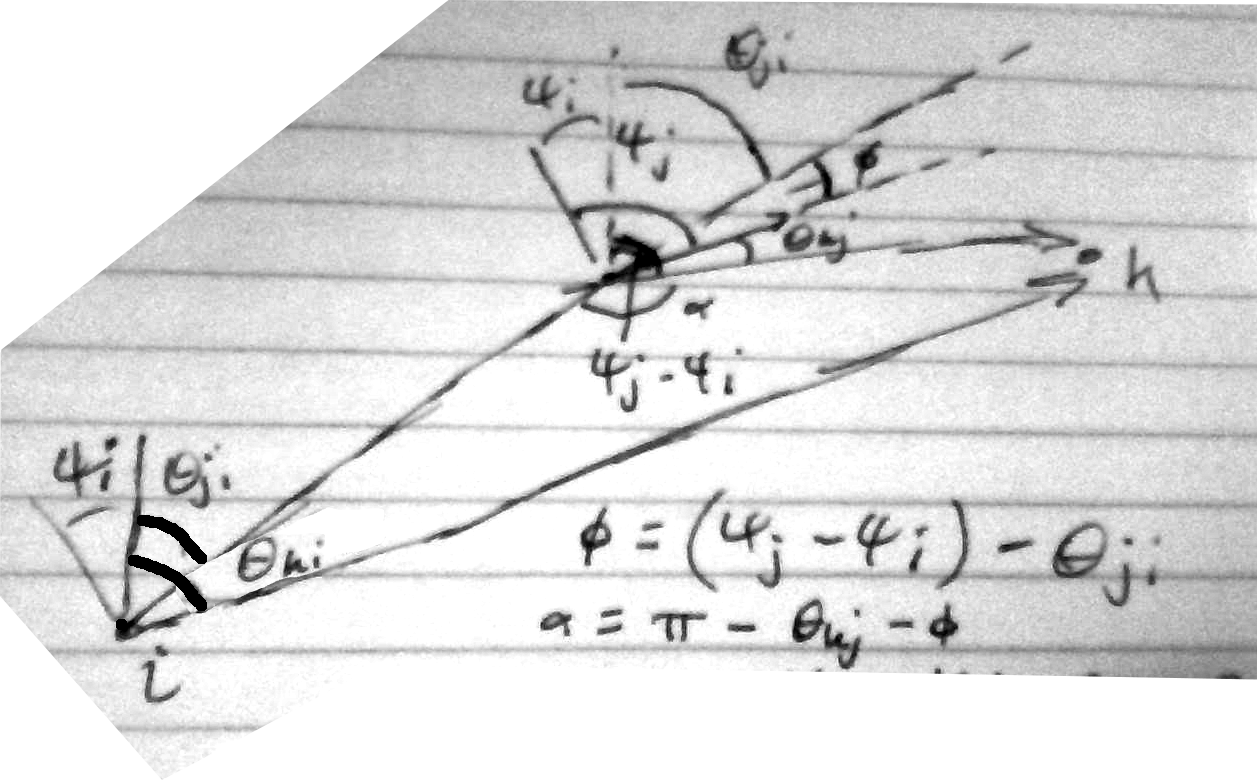
\includegraphics[width=0.75\textwidth]{../cooperative_triangle.png}
\caption{Depiction of interagent bearing angles and ranges.}
\label{fig:coop_triangle}
\end{figure}

Another relationship yields a solution for $\theta_{ki}$:

\begin{align}
\gamma \equiv \theta_{ki}-\theta_{ji}\\% = \arcsin{ \frac{\rho_{kj}}{\rho_{ki}\sin{\alpha}} } \\
\tan{\gamma} = \frac{ 2\rho_{ji}\rho_{kj}\sin{(\psi_i - \psi_j + \theta_{ji} - \theta_{kj})} }{ \rho_{ji}^2 + \rho_{ki}^2 - \rho_{kj}^2 }
\label{eq:gammaEq}
\end{align}

When agents measure both range and bearing to landmarks, Eqs. \ref{eq:lawCos} and \ref{eq:gammaEq} are nonlinear functions of the feature and inter-agent measurements and the estimated agent headings. The effective measurements for the cooperative case are nonlinear functions of $\rho_{ji}$, $\theta_{ji}$, $\rho_{kj}$, and $\theta_{kj}$, as well as the estimated states $\psi_i$ and $\psi_j$. It is assumed that agent $j$ provides its estimate of $\psi_j$ to agent $i$ along with the associated covariance.

Both Eqs. \ref{eq:lawCos} and \ref{eq:gammaEq} depend on the range and bearing of feature $k$ from agent $j$. When feature ranges are not measured, an additional challenge is introduced. For now, both range and bearing are assumed available.

\subsubsection{Feature range and bearing measured}

When both range and bearing are measured, then the desired output equations are nonlinear functions of the four measured states (two ranges and two bearings) and the estimated headings. The computed measurement $\tilde{\B{y}}$ and its expectation are readily determined. To estimate the effective measurement covariance, the method of statistical linearization employed in unscented Kalman filtering is implemented. For the output vector $\B{y} = f(\B{x}), \ \B{x} \ \in \mathit{R}^n, \ \B{x} \sim N(0,P_x)$, $2n+1$ sigma vectors $\BG{\sigma}_i$ are computed as

\begin{align}
\BG{\sigma}_0 = \B{x} \\
\BG{\sigma}_i = \B{x} + \gamma \sqrt{P_x}, \ i = 1,\dots,n \\
\BG{\sigma}_i = \B{x} - \gamma \sqrt{P_x},\ i = n+1,\dots,2n
\end{align}

$\sqrt{P_x}$ is the $i$th column of the matrix square root. Outputs corresponding to each sigma vector $\B{y}_i = f(\BG{\sigma}_i)$ are computed, and the mean and covariance are given by:

\begin{align}
\bar{\B{y}} = \sum_{i=0}^{2n} W_i^{(m)} \B{y}_i \\
P_y = \sum_{i=0}^{2n} W_i^{(c)} (\B{y}_i-\bar{\B{y}})(\B{y}_i-\bar{\B{y}})^T
\end{align}

The weights and scaling factors are defined as:

\begin{align}
\gamma = \sqrt{n+\lambda} \\
\lambda = \alpha^2 (n+k_f)-n \\
W_0^{(m)} = \lambda/(n+\lambda) \\
W_0^{(c)} = \lambda/(n+\lambda) + (1-\alpha^2 + \beta)  \\
W_i^{(m)} = W_i^{(c)} = 1/(2(n+\lambda)), i > 0
\end{align}

Here, $\alpha$ = .01 is used. $\beta = 2$ and $k_f=0$ are given as conventional values for estimation with Gaussian-distributed $\B{x}$.\cite{gyorgy2014}

$P_x$ is populated using the known sensor errors for the interagent and feature range/bearing, and using the estimate covariance for $\psi_i$ and $\psi_j$. The matrix is diagonal in this formulation.

\subsubsection{Only feature bearing measured}

In this case, $\rho_{kj}$ is not measured and the only (?) reasonable choice is to determine the expected range based on agent $j$'s own position estimate, and treat this estimate and its associated covariance as if they are from range measurements. In this case Eq. \ref{eq:gammaEq} becomes a function of an additional estimated state, which will also introduce covariance with the $\psi_j$ estimate.

\subsubsection{Additionally}

The measurement gradients are computed in MATLAB using symbolic variables, and the resulting expressions are used in the EKF. For speed, the EKF is implemented as fully discrete, using a first-order difference approximation for the derivative of each state.

\section{Simulation results}

Dynamic simulation considers two agents in a field of 50 landmarks. Landmarks are uniformly distributed between $\pm 20$ m from the origin. Agent initial $X$ and $Y $ coordinates are normally distributed variables with $\sigma = 5$ m. Agents follow open-loop trajectories with $r(t) = r(0)+(1+sin(ct))$, $\theta(t) = \theta(0) + \frac{\pi}{20}t$, and $\omega = \pm 0.4$ rad/s. $c = 2.2$. The same open-loop trajectories are used in all the following sections. Agents possess unbiased IMUs that measure acceleration and angular rates in the body frame, relative range and bearing measurements of the other agent, and feature measurements. Each agent has a 30\degree half-angle field of view with feature detection at ranges between 2 and 10 meters.

\subsection{Sample output plots}

Sample estimate error plots and inertial trajectories are shown in Figs. \ref{fig:traj_typ}-\ref{fig:agent_typ}. These are provided for problem familiarization only, and are not intended to be statistically representative. Results were generated using accelerometer and gyroscope variances of $0.05$ and $0.01$, respectively, and all range and bearing variances of $1$ and $0.01$, respectively.

\begin{figure}[h!]
\centering
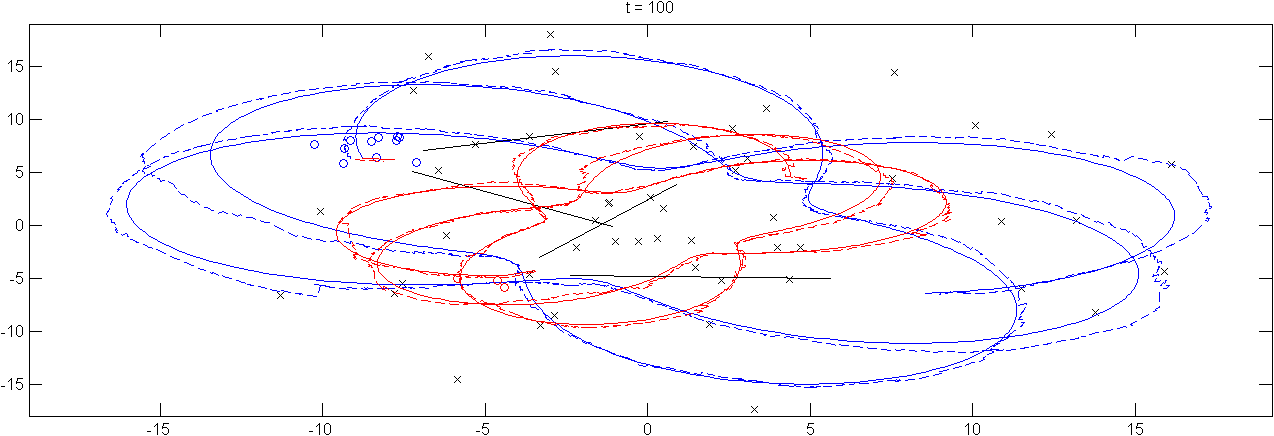
\includegraphics[width=\textwidth]{traj_typ.png}
\caption{Trajectories (solid) for agents 1 and 2 (blue and red, respectively) used in simulation. Dashed lines indicate the estimated trajectory. Features are indicated by ``x''s. Solid black lines, which are hard to see here, indicate the agents' fields of view and minimum and sensitivity extrema. The same data are plotted here as in Fig. \ref{fig:agent_typ}.}
\label{fig:traj_typ}
\end{figure}

\begin{figure}[h!]
\centering
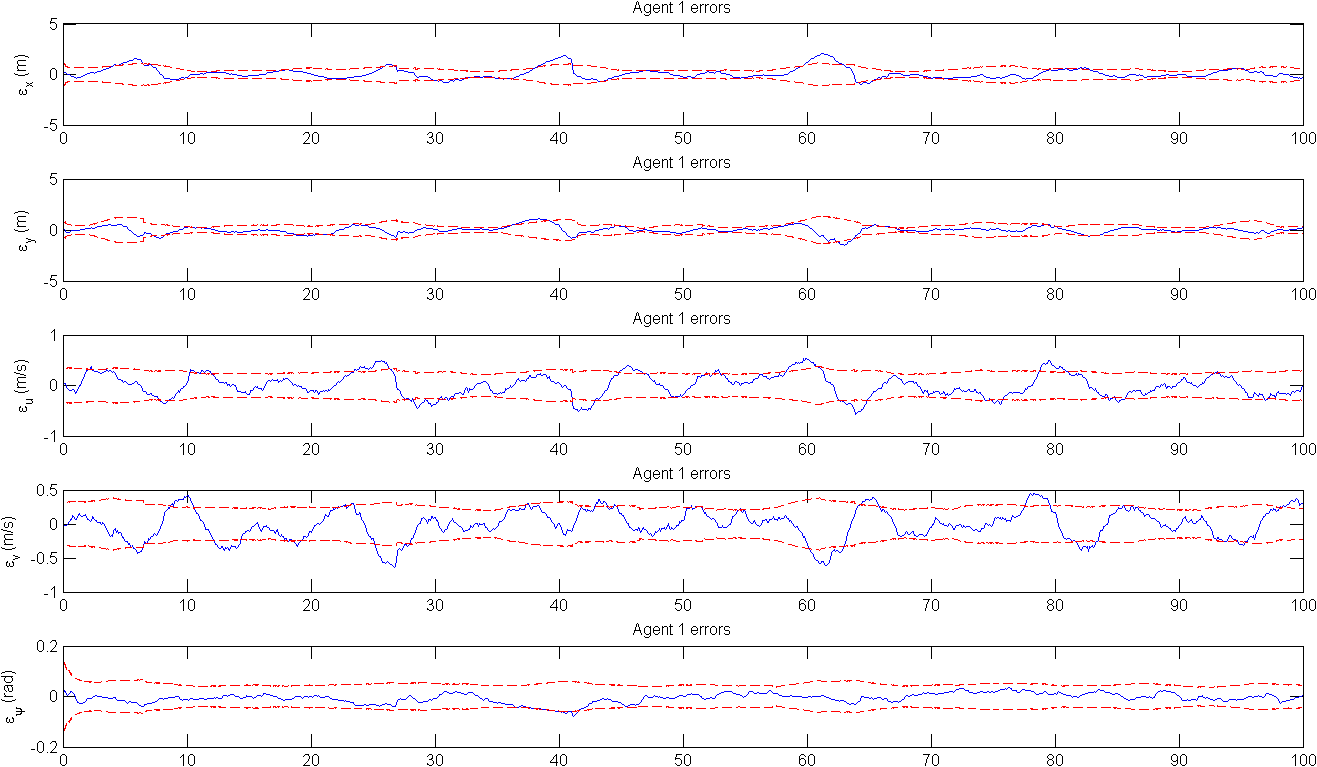
\includegraphics[width=\textwidth]{agent1_typ.png}
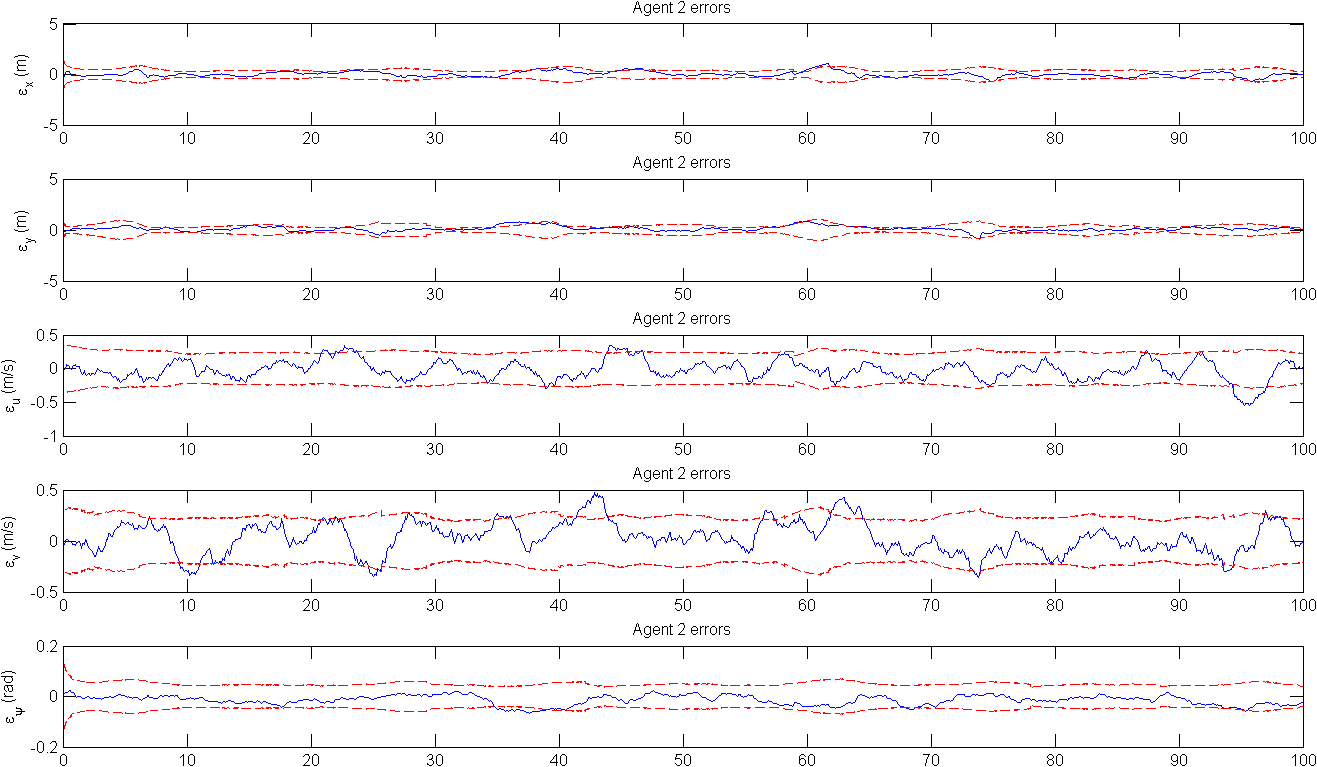
\includegraphics[width=\textwidth]{agent2_typ.png}
\caption{Error histories for agents 1 and 2 from one simulation.}
\label{fig:agent_typ}
\end{figure}

\subsection{Feature range and bearing measured, preliminary results}

This section considers four sets of batch simulations. Each batch consists of 100 repetitions of the same scenario, with new sensor noise generated for each repetition. In each case, the IMU covariance matrix is 

\begin{equation}
R_{imu} = \mathrm{diag}(\begin{bmatrix}
.25 & .25 & .01
\end{bmatrix})
\end{equation}

The interagent bearing measurements have variance $0.01$, and feature range and bearing have variance $10$ and $0.01$ respectively. The four cases consider two different interagent range variance levels $\sigma_{ar}^2$, and two different assumptions for heading accuracy.

\begin{enumerate}
\item $\sigma_{ar}^2 = 1$, true heading is known
\item $\sigma_{ar}^2 = 1$, heading is estimated
\item $\sigma_{ar}^2 = 10$, true heading is known
\item $\sigma_{ar}^2 = 10$, heading is estimated
\end{enumerate}

Results are presented in Tables \ref{tab:case1}-\ref{tab:case4}. These tables list the standard error $S$ and mean squared error ($MSE$) for each state across the 100 simulations in each case. For the case with the low-variance feature range detector, the use of shared measurements benefits agent 1 but not agent 2 in terms of position accuracy. This applies independent of whether heading is known or estimated, although performance is actually slightly better in the simulations with estimated heading. The different performance for the two agents reflects the path-dependence of the cooperative process.

When the range detection has a larger variance, the use of cooperation reduces overall estimation accuracy. This confirms that sufficiently large uncertainties can ``corrupt'' an otherwise stable estimator. The errors are not always lower when the true heading is known, but usually are, which suggests that the use of estimates in the measurement model is a possible source of extra bias. The latter issue might be addressed in several ways. If the heading estimate and shared measurements are sufficiently precise, or if independent heading measurements are available, then this issue is not likely to be a problem.

Note also: in the case where the interagent and feature range are both $1$, using heading estimates, there is a clear improvement from cooperation in agent 1's data, and the individual and cooperative results are essentially identical for agent 2. This result was not tabulated in this writeup because it is of little interest besides confirming that, at low enough noise levels, cooperation can be expected at the worst to ``do no harm.''

\begin{table}[tb!]
\scriptsize
\centering
\begin{tabular}{c|c|c|c|c|c|c|c|c|c|c|c|}
Case & Agent & $S(\epsilon_{rix})$ & $S(\epsilon_{riy})$ & $S(\epsilon_{u})$ & $S(\epsilon_{v})$ & $S(\epsilon_{\psi})$ & $MSE(r_{ix})$ & $MSE(r_{iy})$ & $MSE(u)$ & $MSE(v)$ & $MSE(\psi)$ \\
Individual & 1& 0.779& 0.62& 0.274& 0.258& 0.000501& 0.607& 0.388& 0.0753& 0.0665& 2.51$\times 10^{-7}$ \\
Cooperative & 1& 0.692& 0.623& 0.279& 0.277& 0.0005& 0.495& 0.47& 0.0814& 0.0793& 2.5$\times 10^{-7}$ \\
Individual & 2& 0.357& 0.214& 0.184& 0.162& 0.0005& 0.165& 0.0463& 0.0377& 0.0266& 2.5$\times 10^{-7}$ \\
Cooperative & 2& 0.751& 0.514& 0.293& 0.257& 0.000501& 0.565& 0.268& 0.087& 0.0666& 2.51$\times 10^{-7}$ \\
\end{tabular}
\caption{Case 1 batch simulation results - true heading known with low agent range variance.}
\label{tab:case1}
\end{table}

\begin{table}[tb!]
\scriptsize
\centering
\begin{tabular}{c|c|c|c|c|c|c|c|c|c|c|c|}
Case & Agent & $S(\epsilon_{rix})$ & $S(\epsilon_{riy})$ & $S(\epsilon_{u})$ & $S(\epsilon_{v})$ & $S(\epsilon_{\psi})$ & $MSE(r_{ix})$ & $MSE(r_{iy})$ & $MSE(u)$ & $MSE(v)$ & $MSE(\psi)$ \\
Individual & 1& 0.737& 0.608& 0.258& 0.241& 0.0268& 0.545& 0.37& 0.0676& 0.0579& 0.000931 \\
Cooperative & 1& 0.698& 0.596& 0.276& 0.274& 0.0382& 0.507& 0.487& 0.0812& 0.078& 0.00193 \\
Individual & 2& 0.337& 0.225& 0.177& 0.16& 0.0166& 0.143& 0.054& 0.0355& 0.0257& 0.000309 \\
Cooperative & 2& 0.661& 0.468& 0.262& 0.204& 0.0367& 0.45& 0.246& 0.0692& 0.0462& 0.00194 \\
\end{tabular}
\caption{Case 2 batch simulation results - estimated heading with low agent range variance.}
\end{table}

\begin{table}[tb!]
\scriptsize
\centering
\begin{tabular}{c|c|c|c|c|c|c|c|c|c|c|c|}
Case & Agent & $S(\epsilon_{rix})$ & $S(\epsilon_{riy})$ & $S(\epsilon_{u})$ & $S(\epsilon_{v})$ & $S(\epsilon_{\psi})$ & $MSE(r_{ix})$ & $MSE(r_{iy})$ & $MSE(u)$ & $MSE(v)$ & $MSE(\psi)$ \\
Individual & 1& 0.755& 0.613& 0.274& 0.257& 0.0005& 0.57& 0.38& 0.0755& 0.066& 2.5$\times 10^{-7}$ \\
Cooperative & 1& 0.95& 0.714& 0.317& 0.287& 0.000499& 0.905& 0.614& 0.102& 0.0906& 2.49$\times 10^{-7}$ \\
Individual & 2& 0.353& 0.216& 0.182& 0.163& 0.0005& 0.167& 0.0472& 0.0375& 0.0271& 2.5$\times 10^{-7}$ \\
Cooperative & 2& 0.842& 0.761& 0.346& 0.283& 0.000501& 0.74& 0.619& 0.13& 0.0804& 2.51$\times 10^{-7}$ \\
\end{tabular}
\caption{Case 3 batch simulation results - true heading known with high agent range variance.}
\end{table}

\begin{table}[tb!]
\scriptsize
\centering
\begin{tabular}{c|c|c|c|c|c|c|c|c|c|c|c|}
Case & Agent & $S(\epsilon_{rix})$ & $S(\epsilon_{riy})$ & $S(\epsilon_{u})$ & $S(\epsilon_{v})$ & $S(\epsilon_{\psi})$ & $MSE(r_{ix})$ & $MSE(r_{iy})$ & $MSE(u)$ & $MSE(v)$ & $MSE(\psi)$ \\
Individual & 1& 0.737& 0.611& 0.253& 0.238& 0.0279& 0.545& 0.374& 0.0648& 0.0567& 0.000967 \\
Cooperative & 1& 1.02& 0.744& 0.324& 0.301& 0.0484& 1.04& 0.705& 0.106& 0.102& 0.00341 \\
Individual & 2& 0.355& 0.228& 0.18& 0.159& 0.017& 0.156& 0.0546& 0.0364& 0.0255& 0.000313 \\
Cooperative & 2& 0.736& 0.784& 0.301& 0.248& 0.0555& 0.542& 0.768& 0.0987& 0.0691& 0.00482 \\
\end{tabular}
\caption{Case 4 batch simulation results - estimated heading with high agent range variance.}
\label{tab:case4}
\end{table}

\subsection{Feature range and bearing measured, tuning $\alpha$ parameter}

In this section, the standard error and mean squared error of estimation is considered for different values of the $\alpha$ parameter in statistical linearization. Variances of .01 and 1 are used for all bearing and range measurements, respectively. Tables \ref{tab:alpha1e-4}-\ref{tab:alpha1} show results for $\alpha = .0001$, $\alpha=0.01$, and $\alpha = 1.0$. As before, 100 simulations are performed at each setting. .0001 and 1 were given as typical limits on $\alpha$ by Ref. \citen{gyorgy2014}. The individual agent results are included in these cases to confirm that enough Monte Carlo runs are performed for numerical consistency. Individual results typically agree to two significant figures, indicating reasonably good convergence.

The tabulated results indicate that the errors typically decrease for all states as $\alpha$ increases. The decrease from $\alpha = .0001$ to $.01$ appears to be somewhat larger than from $.01$ to $1$, suggesting diminishing returns at higher values. Since $1$ is given as a typical upper bound in the literature, it is decided not to consider values greater than $1$, in light of potential numerical problems when getting further away from the linearization point.

\begin{table}[tb!]
\scriptsize
\centering
\begin{tabular}{c|c|c|c|c|c|c|c|c|c|c|c|}
Case & Agent & $S(\epsilon_{rix})$ & $S(\epsilon_{riy})$ & $S(\epsilon_{u})$ & $S(\epsilon_{v})$ & $S(\epsilon_{\psi})$ & $MSE(r_{ix})$ & $MSE(r_{iy})$ & $MSE(u)$ & $MSE(v)$ & $MSE(\psi)$ \\
Individual & 1& 0.585& 0.585& 0.221& 0.23& 0.0252& 0.355& 0.345& 0.0491& 0.0533& 0.00116 \\
Cooperative & 1& 0.502& 0.413& 0.234& 0.229& 0.0309& 0.252& 0.171& 0.0548& 0.0527& 0.000968 \\
Individual & 2& 0.243& 0.212& 0.155& 0.154& 0.0169& 0.063& 0.0466& 0.0254& 0.0238& 0.000317 \\
Cooperative & 2& 0.293& 0.336& 0.18& 0.167& 0.0466& 0.0875& 0.116& 0.0336& 0.028& 0.00222 \\
\end{tabular}
\caption{Batch simulation results with $\alpha$ = .0001.}
\label{tab:alpha1e-4}
\end{table}

\begin{table}[tb!]
\scriptsize
\centering
\begin{tabular}{c|c|c|c|c|c|c|c|c|c|c|c|}
Case & Agent & $S(\epsilon_{rix})$ & $S(\epsilon_{riy})$ & $S(\epsilon_{u})$ & $S(\epsilon_{v})$ & $S(\epsilon_{\psi})$ & $MSE(r_{ix})$ & $MSE(r_{iy})$ & $MSE(u)$ & $MSE(v)$ & $MSE(\psi)$ \\
Individual & 1& 0.585& 0.577& 0.217& 0.228& 0.0254& 0.354& 0.336& 0.0474& 0.0523& 0.00116 \\
Cooperative & 1& 0.468& 0.382& 0.231& 0.23& 0.0216& 0.219& 0.146& 0.0538& 0.0529& 0.000474 \\
Individual & 2& 0.244& 0.209& 0.158& 0.155& 0.017& 0.0649& 0.045& 0.0265& 0.0241& 0.000313 \\
Cooperative & 2& 0.248& 0.214& 0.158& 0.154& 0.0169& 0.0631& 0.0478& 0.0259& 0.0236& 0.000338 \\
\end{tabular}
\caption{Batch simulation results with $\alpha$ = .01.}
\label{tab:alpha1e-2}
\end{table}

\begin{table}[tb!]
\scriptsize
\centering
\begin{tabular}{c|c|c|c|c|c|c|c|c|c|c|c|}
Case & Agent & $S(\epsilon_{rix})$ & $S(\epsilon_{riy})$ & $S(\epsilon_{u})$ & $S(\epsilon_{v})$ & $S(\epsilon_{\psi})$ & $MSE(r_{ix})$ & $MSE(r_{iy})$ & $MSE(u)$ & $MSE(v)$ & $MSE(\psi)$ \\
Individual & 1& 0.584& 0.585& 0.221& 0.23& 0.0253& 0.354& 0.344& 0.0491& 0.053& 0.00115 \\
Cooperative & 1& 0.454& 0.373& 0.229& 0.228& 0.0202& 0.206& 0.14& 0.0529& 0.0523& 0.000416 \\
Individual & 2& 0.248& 0.212& 0.157& 0.156& 0.0175& 0.0665& 0.0463& 0.0258& 0.0243& 0.000331 \\
Cooperative & 2& 0.239& 0.202& 0.156& 0.151& 0.0163& 0.0596& 0.0436& 0.0257& 0.0228& 0.000335 \\
\end{tabular}
\caption{Batch simulation results with $\alpha$ = 1.0.}
\label{tab:alpha1}
\end{table}

For further consideration, the Monte Carlo simulations with range variances of 10 are repeated with $\alpha = 1$. These cooperative results, in Table \ref{tab:alpha1_repeat}, are substantially better than those of Table \ref{tab:case4}; the cooperative case is better for agent 1 than the individual case, which was not true in Table \ref{tab:case4}. There is still some loss of accuracy for agent 2 compared to the individual case, but the reduction in performance is greatly lessened compared to the earlier result.

\begin{table}[tb!]
\scriptsize
\centering
\begin{tabular}{c|c|c|c|c|c|c|c|c|c|c|c|}
Case & Agent & $S(\epsilon_{rix})$ & $S(\epsilon_{riy})$ & $S(\epsilon_{u})$ & $S(\epsilon_{v})$ & $S(\epsilon_{\psi})$ & $MSE(r_{ix})$ & $MSE(r_{iy})$ & $MSE(u)$ & $MSE(v)$ & $MSE(\psi)$ \\
Individual & 1& 0.746& 0.62& 0.26& 0.243& 0.0283& 0.558& 0.385& 0.0679& 0.0591& 0.00101 \\
Cooperative & 1& 0.695& 0.518& 0.256& 0.247& 0.0275& 0.483& 0.295& 0.0655& 0.0623& 0.000756 \\
Individual & 2& 0.337& 0.225& 0.174& 0.158& 0.0172& 0.141& 0.0536& 0.0347& 0.0251& 0.000327 \\
Cooperative & 2& 0.419& 0.277& 0.194& 0.165& 0.0227& 0.179& 0.0875& 0.0396& 0.0274& 0.000703 \\
\end{tabular}
\caption{Repeated Monte Carlo with range variance equal to 10 and $\alpha$ = 1.0.}
\label{tab:alpha1_repeat}
\end{table}

\subsection{Heading drift with and without shared measurements}

This section highlights the effect of shared measurements on heading angle estimation. To demonstrate, an exaggerated scenario is considered in which one agent makes no feature measurements of its own and merely receives interagent measurements and measurements made by the other agent. All state estimate errors are initially zero.

\begin{figure}[p!]
\centering
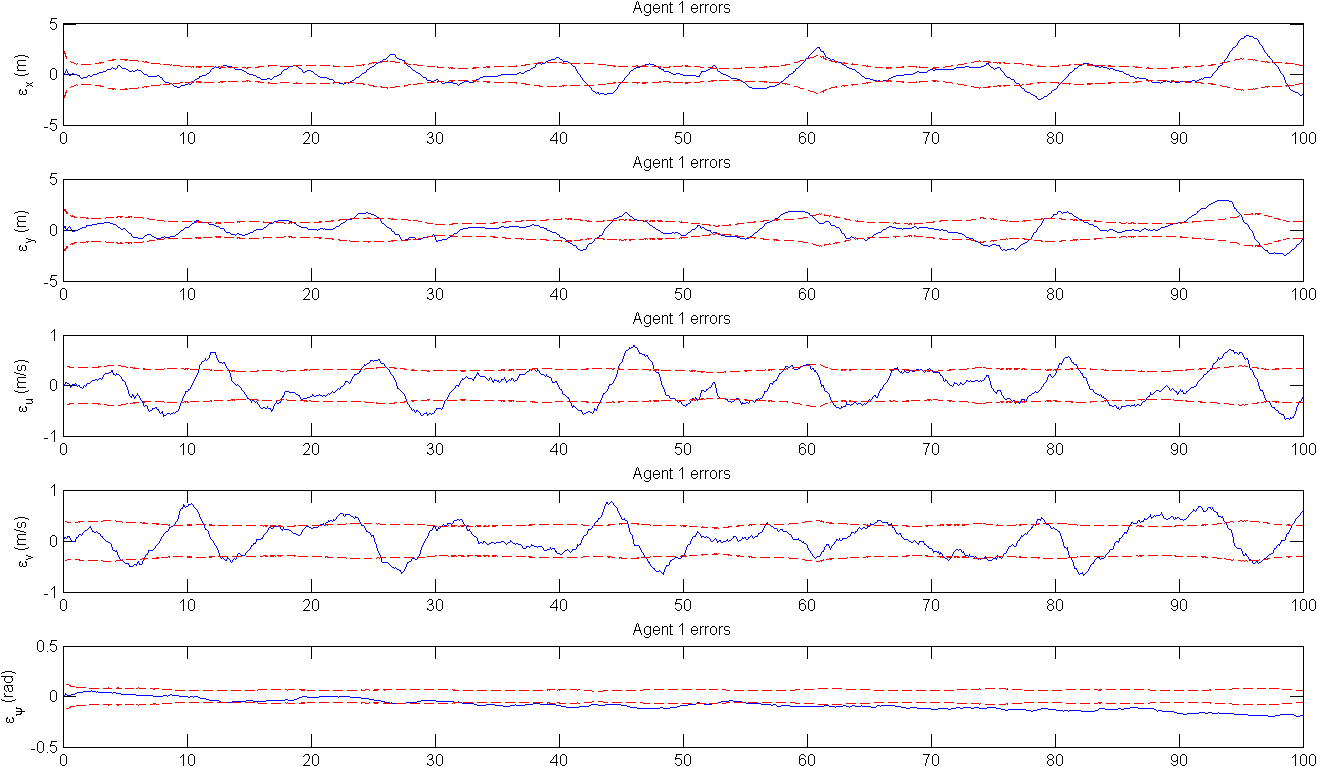
\includegraphics[height=.4\textheight]{heading_drift.png}
\caption{Estimate error time histories for one agent, using only shared and interagent measurements.}
\label{fig:heading_drift}
\end{figure}

\begin{figure}[p!]
\centering
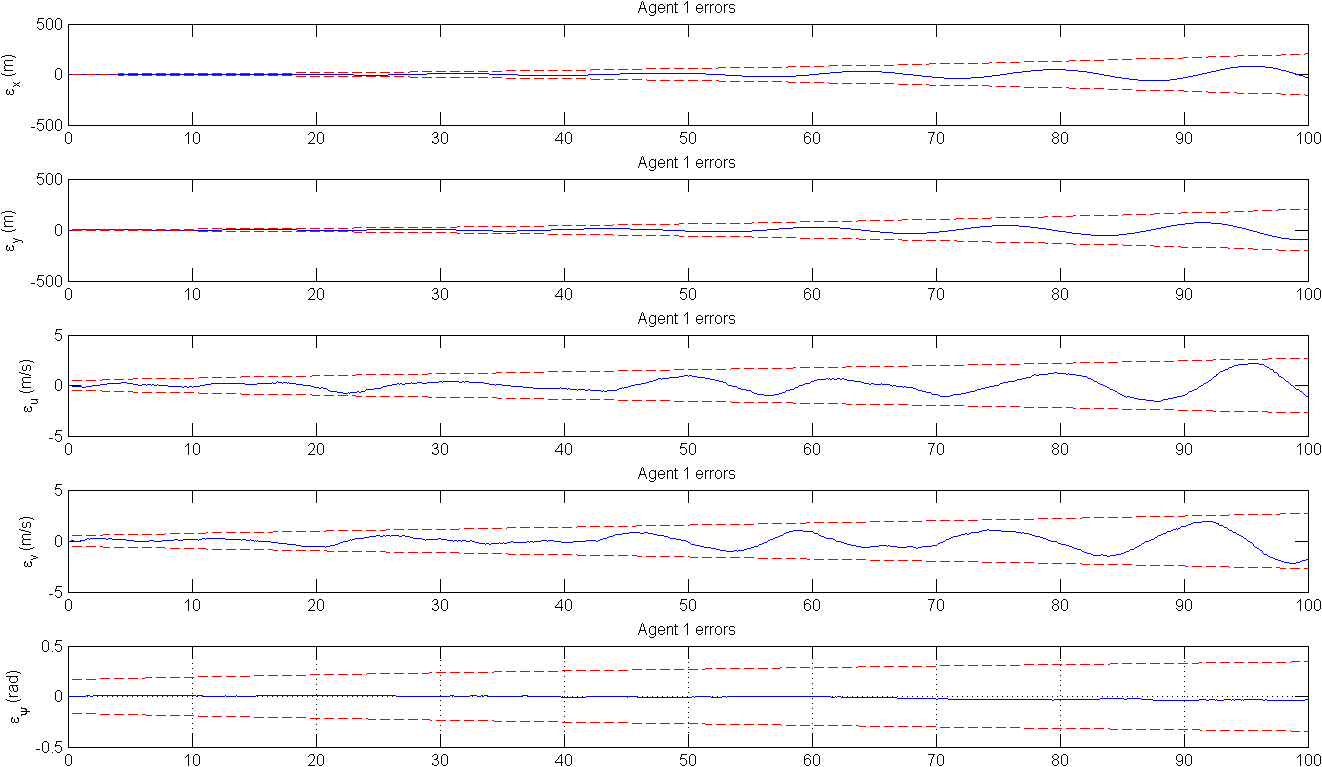
\includegraphics[height=.4\textheight]{heading_drift_nothing.png}
\caption{Estimate error time histories for one agent, using no measurements.}
\label{fig:heading_drift_nothing}
\end{figure}

Fig. \ref{fig:heading_drift} shows the estimate error time histories for this ``blind'' agent, with the associated covariance $3\sigma$ bounds. The position and velocity state estimates remain bounded (although not necessarily by the $3\sigma$ value), but the heading angle appears to drift without correction. The error is defined as the estimate minus the truth, and the heading angle estimate error is steadily growing more negative as time passes. This result was recorded when the agent was rotating in the direction of increasing $\psi$. This implies that the estimate grew more slowly than the truth value, and this was observed over several consecutive single simulations.

Fig. \ref{fig:heading_drift_nothing} further highlights the effect of using shared measurements only. In the figure that produced this simulation, no measurements were used by this agent to update its estimates. As expected, the covariance for all three axes grows unbounded. However, the heading angle estimate has a very small error, on the order of 0.01 rad. This error order of magnitude was observed across several consecutive single simulations, suggesting a trend. Since the yaw rate gyroscope has a lower variance than the accelerometers, this relatively slow drift in heading angle from pure integration of the gyros is not surprising. Comparison of Figs. \ref{fig:heading_drift} and \ref{fig:heading_drift_nothing} highlights the extreme case of the influence of sharing feature measurements. Without some kind of egocentric feature measurements, the agent that depends on shared feature measurements will experience a heading angle drift that is much more severe than the error from the gyros alone. It is important to note that the other agent states are still stabilized by using the shared measurements. There may be ways to maneuver the sharing agent so as to mitigate this drift on the ``blind'' agent's heading.

\subsection{Effect of shared measurement update rate}

In this section, the effect of reducing the frequency with which shared measurements are available is considered. Previously, IMU and both shared and egocentric feature measurements were available at 10 Hz. In this section, we consider the same simulation settings as those of Table \ref{tab:alpha1}, except with shared measurements only available at 1 Hz and .1 Hz.

Table \ref{tab:1Hz} shows errors with 1 Hz measurement sharing. The errors in the cooperative case are between those of Table \ref{tab:alpha1} and the individual case. As with a 10 Hz sharing, agent 2 has lower errors in the cooperative case, but the improvement is small enough to be negligible in many practical environments. However, agent 1 still performs substantially better in the cooperative case compared to the individual case, although not as well as with 10 Hz sharing.

\begin{table}[tb!]
\scriptsize
\centering
\begin{tabular}{c|c|c|c|c|c|c|c|c|c|c|c|}
Case & Agent & $S(\epsilon_{rix})$ & $S(\epsilon_{riy})$ & $S(\epsilon_{u})$ & $S(\epsilon_{v})$ & $S(\epsilon_{\psi})$ & $MSE(r_{ix})$ & $MSE(r_{iy})$ & $MSE(u)$ & $MSE(v)$ & $MSE(\psi)$ \\
Individual & 1& 0.59& 0.581& 0.216& 0.227& 0.0253& 0.361& 0.34& 0.0472& 0.0518& 0.0012 \\
Cooperative & 1& 0.519& 0.5& 0.22& 0.224& 0.0231& 0.278& 0.251& 0.0484& 0.0503& 0.000858 \\
Individual & 2& 0.248& 0.22& 0.157& 0.155& 0.0175& 0.0661& 0.0494& 0.0259& 0.024& 0.000332 \\
Cooperative & 2& 0.247& 0.211& 0.156& 0.153& 0.017& 0.0648& 0.046& 0.0255& 0.0236& 0.000324 \\
\end{tabular}
\caption{Monte Carlo simulations with range variance equal to 10 and 1 Hz measurement sharing.}
\label{tab:1Hz}
\end{table}

Table \ref{tab:.1Hz} shows Monte Carlo results for the same settings with a 0.1 Hz measurement sharing. Agent 2 performs almost identically in the shared and individual scenarios, and the performance at 1 Hz and 0.1 Hz is essentially indistinguishable. Agent 1 performs a little better in the cooperative case than in the individual one, but the improvement is much less than at previous settings. 0.1 Hz is probably approaching a point of diminishing returns for shared measurements. It should be noted that the performance of sharing at low rates is approaching the individual performance, so the low-rate sharing is not corrupting performance here. 

We have shown that lower sharing rates can still be beneficial. It is likely that the lower limit of allowable sharing will be highly dependent on the exact sensor noise levels. It should also be noted that there is potentially an element of path dependence here; if one of the agents consistently is not observing features at a multiple of the sharing frequency, it may derive much more benefit from sharing than is realistic at a given rate.

\begin{table}[tb!]
\scriptsize
\centering
\begin{tabular}{c|c|c|c|c|c|c|c|c|c|c|c|}
Case & Agent & $S(\epsilon_{rix})$ & $S(\epsilon_{riy})$ & $S(\epsilon_{u})$ & $S(\epsilon_{v})$ & $S(\epsilon_{\psi})$ & $MSE(r_{ix})$ & $MSE(r_{iy})$ & $MSE(u)$ & $MSE(v)$ & $MSE(\psi)$ \\
Individual & 1& 0.586& 0.585& 0.217& 0.228& 0.0247& 0.355& 0.345& 0.0472& 0.0524& 0.00108 \\
Cooperative & 1& 0.576& 0.563& 0.219& 0.228& 0.0242& 0.343& 0.319& 0.0485& 0.0521& 0.00109 \\
Individual & 2& 0.248& 0.222& 0.159& 0.155& 0.0175& 0.0651& 0.0501& 0.0262& 0.0241& 0.000338 \\
Cooperative & 2& 0.246& 0.216& 0.157& 0.155& 0.0175& 0.0651& 0.0481& 0.0261& 0.0241& 0.000339 \\
\end{tabular}
\caption{Monte Carlo simulations with range variance equal to 10 and 0.1 Hz measurement sharing.}
\label{tab:.1Hz}
\end{table}

\pagebreak
\section{Summary}

Primary findings:

\begin{itemize}
\item Measurement sharing in two dimensions can improve estimation accuracy, although performance depends highly on the available sensor variances.
\item Sharing inaccurate measurements can ``corrupt'' estimators and reduce performance. This effect is likely partly or entirely related to the treatment of heading angle estimates as measured values in the utilization of shared measurements.
\item Use of statistical linearization offers some improvement in estimator accuracy, and presumably in covariance estimation, compared to analytical methods using the Jacobian of a measurement vector. This effect was not detailed in this document but was explored in simulation. Improved performance for larger values of the parameter $\alpha$ suggests the statistical method better captures nonlinearities by considering sigma points further from the linearization point.
\item Use of shared feature measurements can have a significant effect on agent heading estimates. In the extreme case when an agent only has access to feature measurements from another agent, sequential heading angle estimates in general can drift much faster than they would from IMU integration alone. Position and velocity estimates appear to remain bounded. Use of a batch estimator as a backend could mitigate this effect.
\item The rate at which measurements are shared may be reduced somewhat while still improving estimate accuracy compared to the individual case. The lower limit of the rate for useful sharing likely depends highly on the sensor variance levels and is not thoroughly explored in this document. In one scenario, it was found that reduction of the sharing rate by an order of magnitude still offered some improvement over the no-sharing case, but reduction by two orders of magnitude offered essentially no benefit.
\end{itemize}

\bibliography{../../references}
\bibliographystyle{aiaa}

\end{document}
